% Responsável: P1 (corpus) + P5 (anotação)
\section{Dados}\label{sec:dados}

\paragraph{Origem e licença.}
O Fake.Br~\cite{monteiro2018} contém 7\,200 notícias em português do Brasil: 3\,600 falsas e
3\,600 verdadeiras. Segundo os autores, as falsas foram recolhidas em sítios que as agregam e,
para cada uma, foi procurada manualmente uma notícia verdadeira sobre o mesmo assunto em jornais de
referência, formando pares. As notícias foram recolhidas entre janeiro de 2016 e janeiro de
2018~\cite{santos2020}. O corpus é
distribuído num repositório público\footnote{\url{https://github.com/roneysco/Fake.br-Corpus}}
que \textbf{não inclui ficheiro de licença}; os autores pedem apenas a citação dos artigos.
Usamo-lo para investigação, sem redistribuir os textos: o nosso código descarrega-o num
\emph{commit} fixo (\texttt{780f551}).

\paragraph{Estrutura.}
Cada notícia tem duas versões: o texto completo e uma versão em que o texto mais longo de cada
par foi cortado ao comprimento do mais curto. Acompanham-na 25 metadados (autor, ligação, categoria,
data e atributos linguísticos calculados pelos autores). Os temas são muito desequilibrados:
política (58\%), TV e celebridades (21\%), sociedade e quotidiano (18\%), e três temas pequenos
(ciência e tecnologia, economia, religião) que agregámos em ``outros'' (3\%).

\begin{table}[t]\centering\small
\caption{Estatísticas descritivas do conjunto de desenvolvimento (2\,878 pares).}\label{tab:corpus}
\begin{tabular}{lrr}
\toprule
& Verdadeiras & Falsas \\
\midrule
Documentos & 2 878 & 2 878 \\
Palavras (total) & 3 170 854 & 528 398 \\
Palavras por doc.\ (mediana) & 919 & 156 \\
\quad percentil 10 & 439 & 83 \\
\quad percentil 90 & 1 987 & 306 \\
Palavras, versão normalizada (mediana) & 157,5 & 155,0 \\
Palavras em maiúsculas (mediana) & 9 & 3 \\
Erros ortográficos (\%, média) & 0,22 & 0,38 \\
Palavras por frase (mediana) & 20,6 & 14,9 \\
Domínio mais frequente (\% da classe) & 64,3 & 92,7 \\
\bottomrule
\end{tabular}\par\smallskip{\footnotesize Metadados de estilo calculados pelos autores do corpus sobre o texto completo.}
\end{table}


\paragraph{Dificuldades.}
A Tabela~\ref{tab:corpus} e uma análise dos finais dos textos mostram quatro problemas que condicionam todo o trabalho.
(1)~\emph{Viés de comprimento}: as verdadeiras têm mediana de 919 palavras e as falsas de 156;
na versão normalizada as medianas ficam em 158 e 155. (2)~\emph{Viés de fonte}: 92,7\% das falsas
do conjunto de desenvolvimento vêm de um único domínio e 64,3\% das verdadeiras do G1.
(3)~\emph{Ruído e duplicação}: 17 notícias verdadeiras aparecem em mais do que um par (mesma
ligação), quatro ficheiros da versão normalizada não correspondem aos da versão completa
(numeração diferente) e as datas surgem em formatos heterogéneos. As falsas têm em média mais
erros ortográficos (0,38\% vs.\ 0,22\%) e frases mais curtas (14,9 vs.\ 20,6 palavras).
(4)~\emph{Artefacto de truncagem}: a versão normalizada, criada para remover o viés de comprimento,
cria outro. Como é quase sempre a verdadeira que é mais longa, 98\% das verdadeiras foram cortadas a
meio de uma frase, e só 7\% acabam em pontuação, contra 77\% das falsas. Quatro atributos sobre o
último carácter dão F1-macro de 0,890 (Tabela~\ref{tab:cv}). Criámos por isso uma terceira versão,
\emph{cortada}: as primeiras 100 palavras do texto normalizado (ou todas menos as 5 últimas, nos
textos mais curtos), de modo que \emph{todos} os textos terminam a meio e a mesma
\emph{baseline} desce para 0,395.

\paragraph{Lei de Zipf.}
A Figura~\ref{fig:zipf} mostra a frequência das palavras em função da ordem, em escala log-log.
Ajustando uma reta nas ordens 10 a 10\,000 obtemos $\alpha=1{,}130$ para as verdadeiras e
$\alpha=1{,}122$ para as falsas, próximos do valor clássico $\alpha\approx1$~\cite{zipf1949,piantadosi2014}.
As duas classes seguem a lei de forma quase idêntica; a diferença de vocabulário (74\,782 vs.\ 30\,804
tipos) resulta sobretudo da diferença de volume de texto. Cerca de 40\% do vocabulário são
\emph{hapax legomena}, o que justifica ignorar termos que ocorrem num só documento.

\begin{figure}[t]\centering
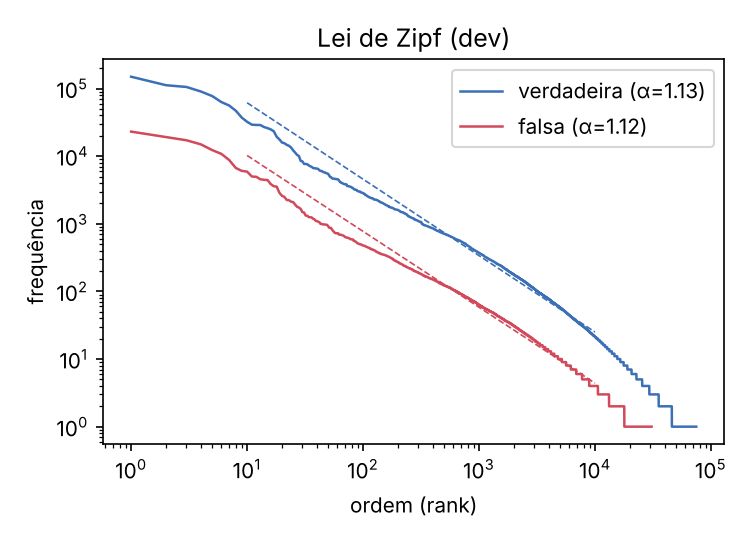
\includegraphics[width=0.48\linewidth]{figs/zipf.png}\hfill
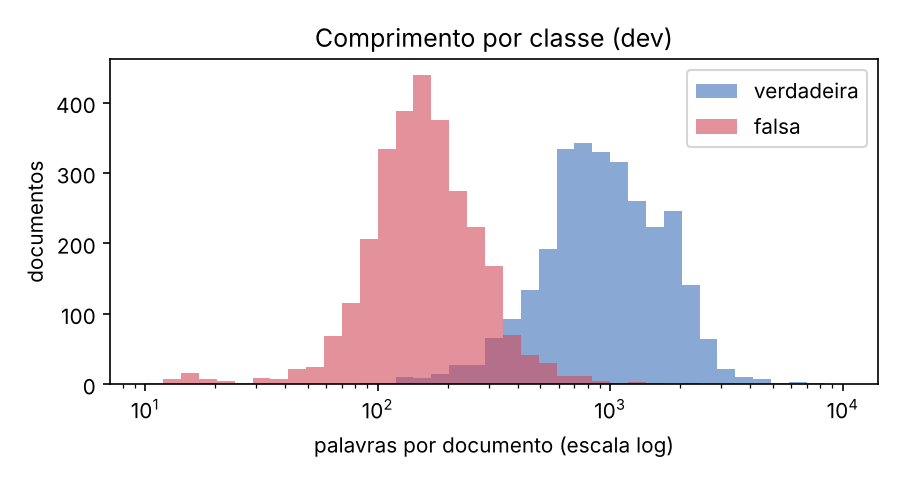
\includegraphics[width=0.48\linewidth]{figs/comprimento.png}
\caption{Esquerda: lei de Zipf por classe (dev), com a reta ajustada. Direita: distribuição do
comprimento por classe (escala logarítmica), que evidencia o viés de comprimento.}\label{fig:zipf}
\end{figure}

\paragraph{Anotação manual para a extração de informação.}
Selecionámos 50 pares (100 notícias) do conjunto de desenvolvimento, estratificados por tema,
usando o texto normalizado. Os anotadores não conhecem o rótulo de cada notícia (códigos opacos,
ordem aleatória) nem usam ferramentas de pré-anotação. Anotam quatro tipos: pessoa, organização,
local e data, segundo um guia com regras e exemplos (no repositório). Vinte notícias foram
anotadas por dois anotadores, para medir a concordância. Uma limitação: como os textos normalizados
das verdadeiras acabam quase sempre a meio de uma frase, o corte pode sugerir a classe ao anotador;
as regras de anotação não dependem da classe, e os anotadores foram instruídos a ignorá-la.
Ao longo da anotação surgiram casos não previstos (títulos como ``Dona'' ou ``Papa'', hospitais e
fazendas, partidos com a sigla do estado, horas), decididos em grupo e acrescentados ao guia antes de
todos terminarem. Os cinco anotadores produziram 931 entidades distintas no ouro principal. Nas 20
notícias com dupla anotação, a concordância (F1 entre anotadores) é de 0,875 com correspondência
estrita e 0,931 relaxada; é mais baixa nas datas (0,708 estrita, 0,958 relaxada), sobretudo por
diferenças na extensão da expressão (``quinta-feira, 18'' vs.\ ``quinta-feira''), e nas organizações
(0,816). Não houve adjudicação: o ouro de cada notícia é o do anotador principal. Uma verificação
automática de formato encontrou 10 inconsistências (cerca de 1\%: erros de cópia, como ``Mendonza''
por ``Mendoza'', e números de dia anotados sozinhos), que mantivemos como parte do ruído da anotação.
